\subsubsection{Pushbutton Key Parallel Port}

The parallel port connected to the {\it KEY}$_{3-1}$ 
pushbutton switches on the \DEBoard~board comprises three 3-bit
registers, as shown in Figure \ref{fig:pushbutton_port}. These registers have 
the base addresses {\sf 0xFF200050} and can be accessed using word operations. 
The read-only {\it Data} register provides the 
values of the switches {\it KEY}$_3$, {\it KEY}$_2$ and {\it KEY}$_1$. Bit 0 of the 
{\it Data} register is not used, because the corresponding switch {\it KEY}$_0$ is reserved for
use as a reset mechanism for the \systemName.
The other two registers shown in Figure \ref{fig:pushbutton_port}, at addresses
{\sf 0xFF200058} and {\sf 0xFF20005C}, are discussed in Section \ref{sec:exceptions}.
~\\
~\\
\begin{figure}[h!]
   \begin{center}
       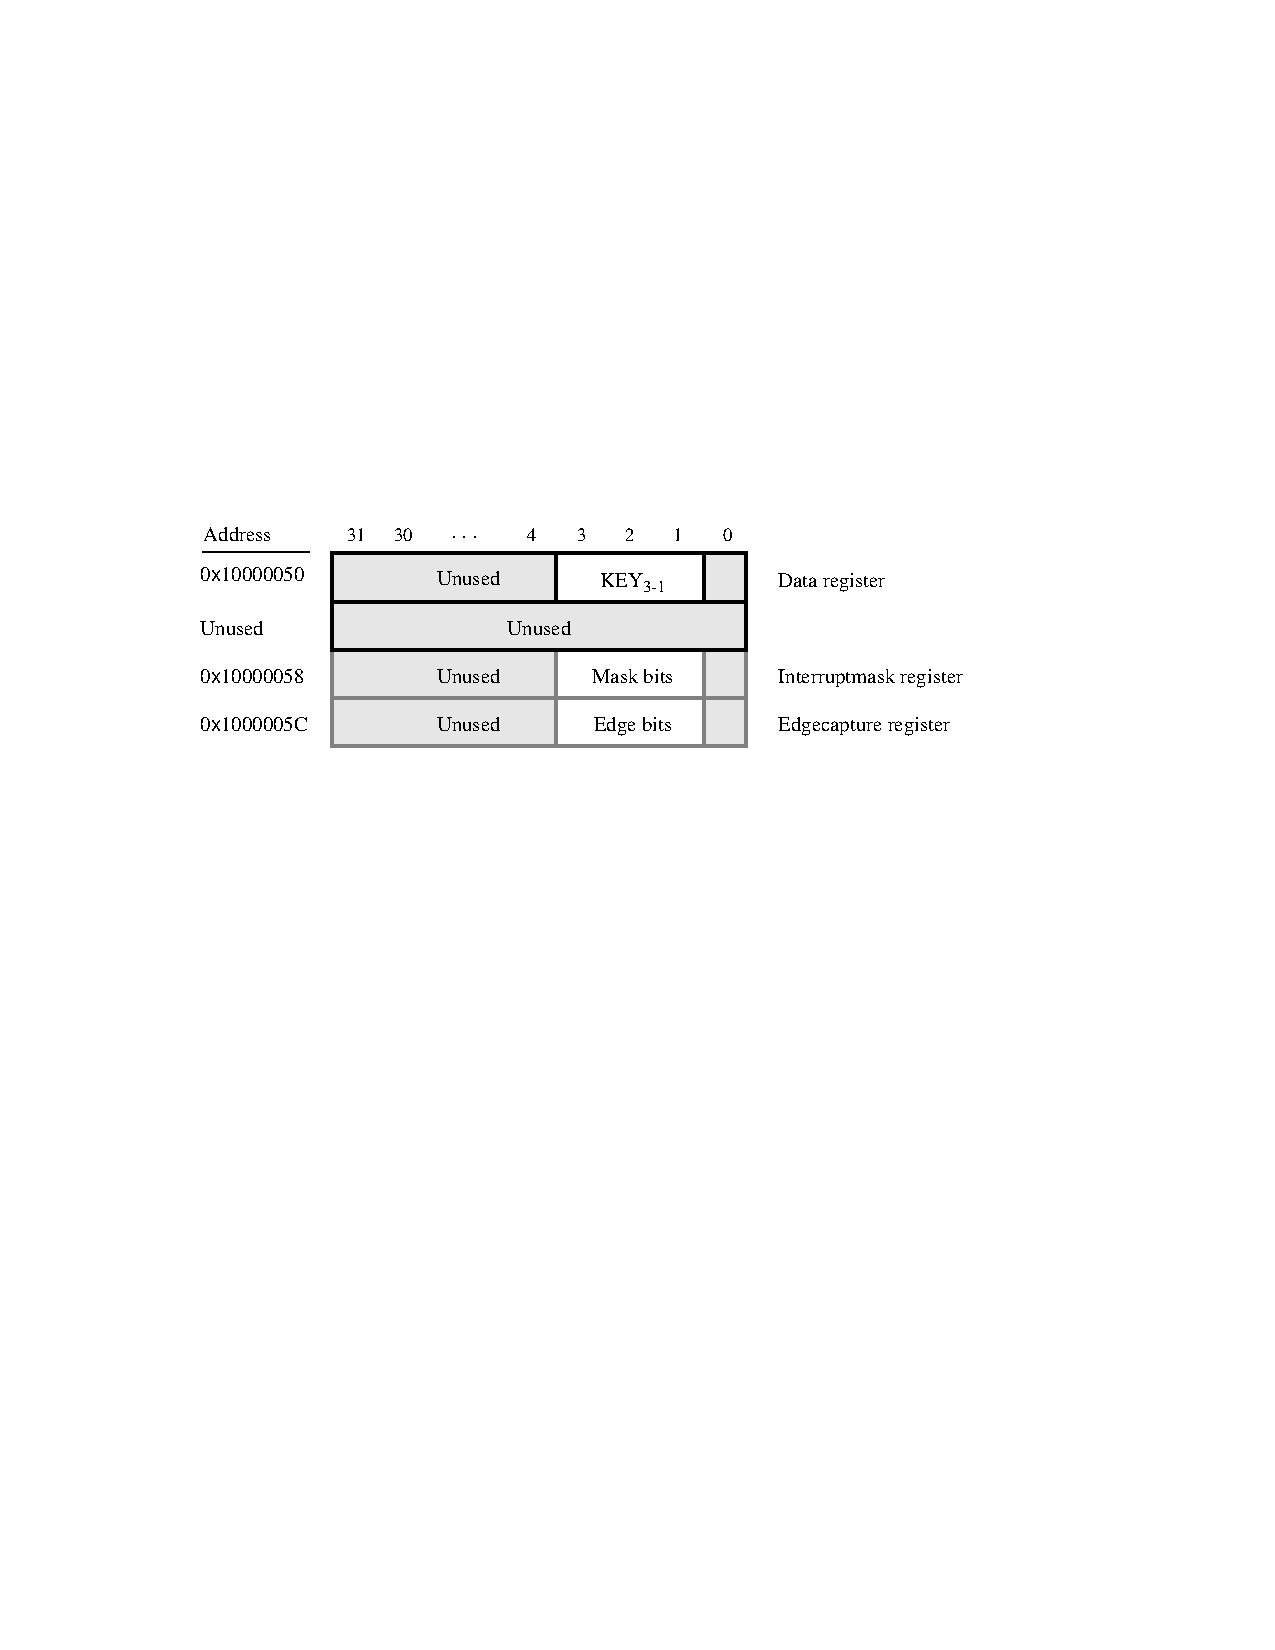
\includegraphics{../../../common/figs/FPGA_PP_Keys_3.pdf}
   \end{center}
   \caption{Registers used in the pushbutton parallel port.}
	\label{fig:pushbutton_port}
\end{figure}
